\section{Modell Anpassungen}
Das trainierte Modell der Walker Demo beherrscht jedoch nur die Fortbewegung in Blickrichtung. Der Läufer ist auch nicht darauf trainiert stehen zu bleiben. Das resultiert darin das der Läufer fällt sobald der Nutzer keinen Tastaturinput gibt. Dieses Kapitel beschäftigt sich mit den Einschränkungen der Walker-Demonstration im Bezug auf unterschiedliche Bewegungsrichtungen.

Im ersten Schritt wird getestet wie der Walker angepasst werden kann um die fehlenden Bewegungsabläufe in separaten Modellen zu erlernen.

\subsection{Versuch 4}
Versuch 4 behandelt die Bewegung auf der Stelle stehen. Für das stehenbleiben wird die Zielgeschwindigkeit auf 0 gesetzt während das Ziel auf der Startposition befindet. Die Belohnungsfunktion der Demo, wird ab jetzt Demo Belohnungsfunktion genannt. Die Demo Belohnungsfunktion hat das Problem das durch die Zielgeschwindigkeit geteilt wird, was bei einer Zielgeschwindigkeit von 0 zu Mathematischen Fehlern führt. Um das zu vermeiden wurde das trainieren mit einer anderen Belohnungsfunktion getestet.
\begin{figure}[H]
  \centering  
  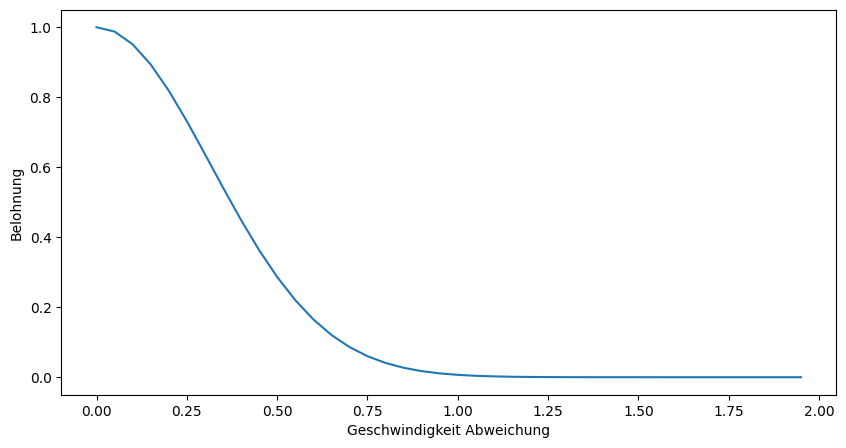
\includegraphics[scale=0.5]{img/match_velocity_exp.png}
  \caption{DeepMimic Match Velocity Belohnungsfunktion}
  \label{fig:match_velocity_exp}
\end{figure}
Die neue Belohnungsfunktion ist inspiriert von den Belohnungsfunktionen des Papers "DeepMimic: Example-Guided Deep Reinforcement Learning of Physics-Based Character Skills".\cite{peng2018deepmimic}
Die Belohnungsfunktion aus Abbildung \ref{fig:match_velocity_exp} wird daher ab hier DeepMimic Belohnungsfunktion genannt.

Der Walker konnte mit der DeepMimic Belohnungsfunktion lernen auf der Stelle zu stehen. Mit zufälliger Zielgeschwindigkeit zu einem Ziel zu laufen wie im Ursprünglichen Verhalten konnte damit jedoch nicht zufriedenstellend erlernt werden.

\begin{figure}[H]
  \centering  
  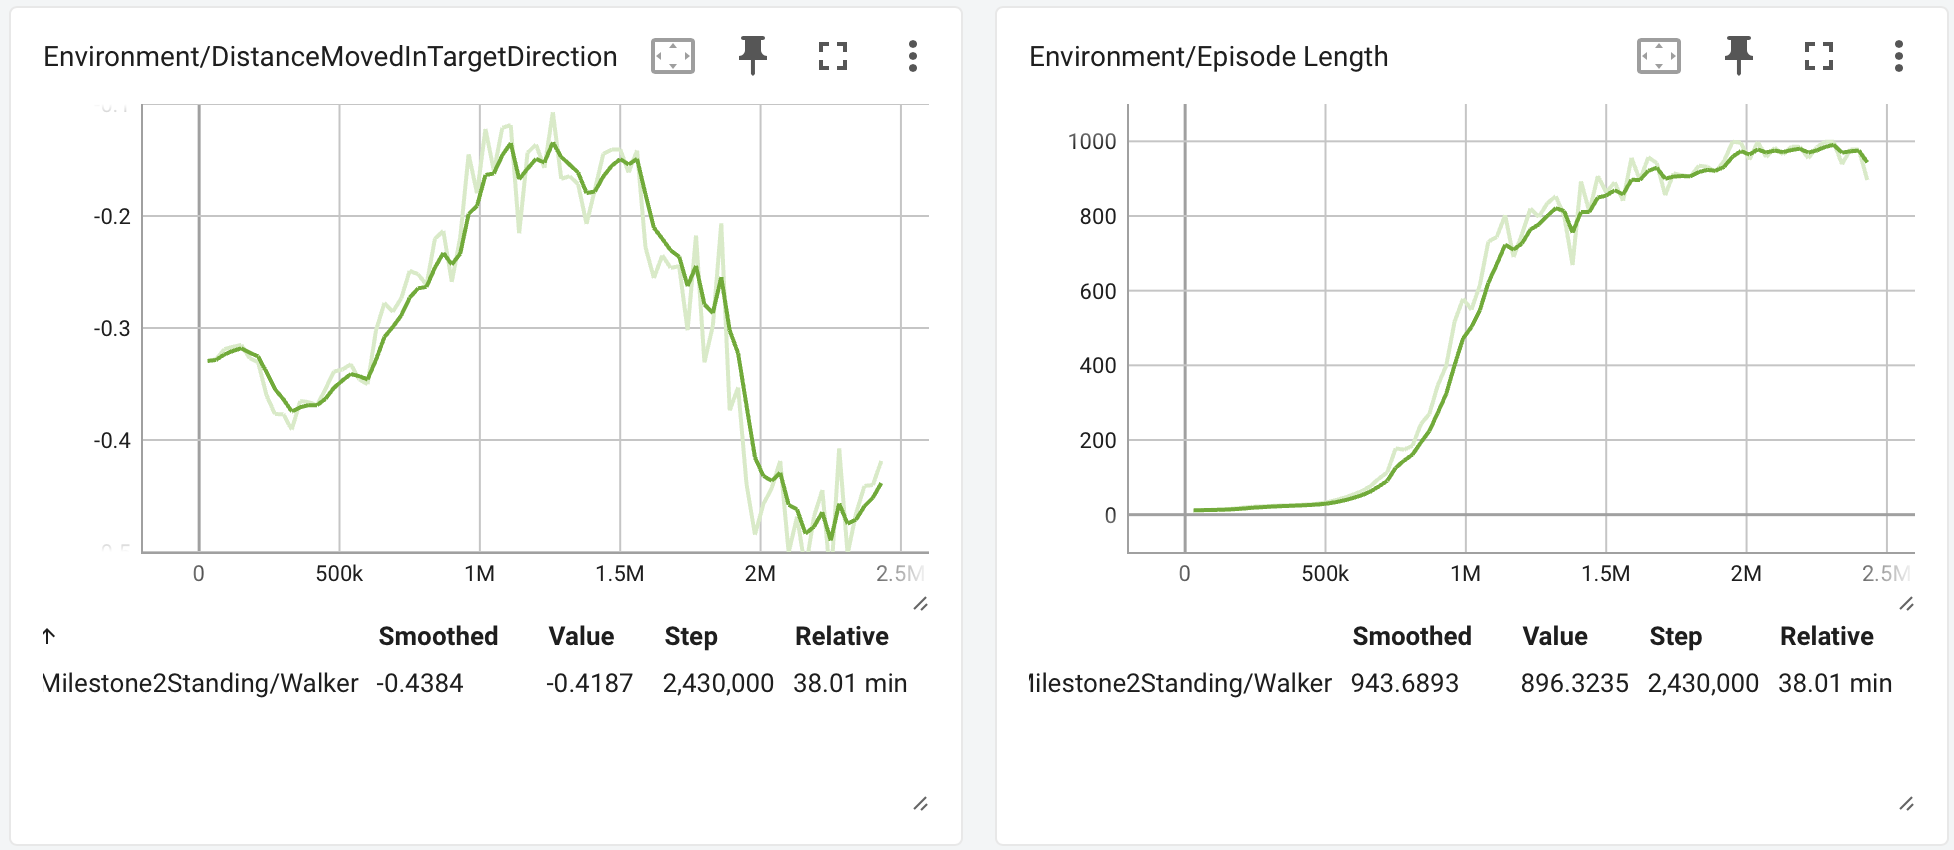
\includegraphics[scale=0.5]{img/versuch4_training}
  \caption{Vergleich von Training mit Demo Belohnungsfunktion gegen DeepMimic Belohnungsfunktion}
  \label{fig:versuch4_training}
\end{figure}

Die Abbildung \ref{fig:versuch4_training} zeigt mit der orangenen Linie die Leistung der DeepMimic Belohnungsfunktion und mit der pinken Linie die Leistung der Demo Belohnungsfunktion. Nachfolgender Vergleich der Belohnungsfunktionen zeigt das die Ursprüngliche Belohnungsfunktion durch das Teilen mit der Zielgeschwindigkeit die Sensitivität der Funktion je nach Zielgeschwindigkeit beeinflusst. Daraus folgt das bei steigender Zielgeschwindigkeit eine größere Abweichung der Geschwindigkeit geduldet wird (siehe Abbildung \ref{fig:match_velocity_demo_vergleich}). Diese Anpassung verbessert die Generalisierung zwischen den wechselnden Geschwindigkeiten um ein vielfaches.

\begin{figure}[H]
  \centering  
  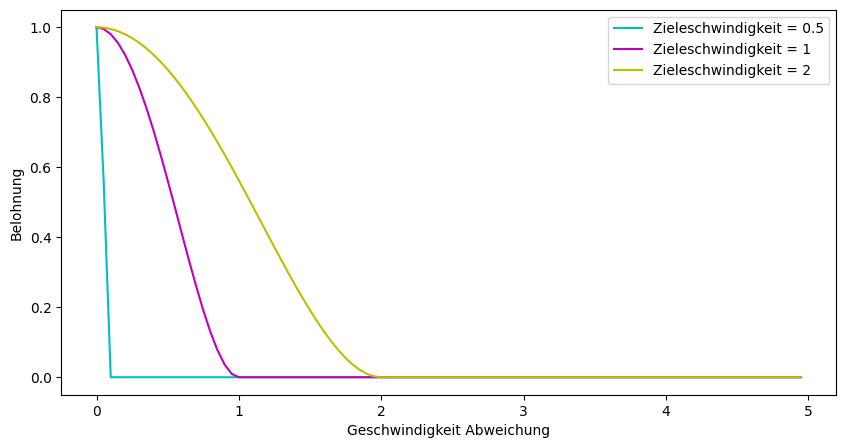
\includegraphics[scale=0.5]{img/match_velocity_demo_vergleich.png}
  \caption{Vergleich der Demo Belohnungsfunktion unter verschiedenen Zielgeschwindigkeiten}
  \label{fig:match_velocity_demo_vergleich}
\end{figure}

\subsection{Versuch 5}
Mit dieser Erkenntnis wurde eine neue Anpassung untersucht. In der folgenden Anpassung blieb die Belohnungsfunktion weitestgehend Unverändert. Lediglich das obere Limit ab welchem die Funktion eine Belohnung von 0 annimmt, wurde auf ein minimum von 0.1 beschränkt. Somit konnte sicher gestellt werden das im Bereich der normalen Fortbewegung keine Veränderung auftritt. Mit der Demo Belohnungsfunktion konnten nur Annäherungen an eine Zielgeschwindigkeit von 0 genutzt werden. Bei einer Annäherung von 0.000001 ist das Spektrum an akzeptablen Geschwindigkeiten bevor die Belohnung 0 ist nahezu unerreichbar (siehe Abbildung \ref{fig:match_velocity_vergleich_clip}). Mit dem Limit von 0.1 ist der Bereich der Belohnungsfunktion > 0 groß genug, sodass der Läufer durch ausprobieren Belohnungen über 0 erreichen kann. Somit kann der Läufer die Belohnung optimieren.\\

\begin{figure}[H]
  \centering  
  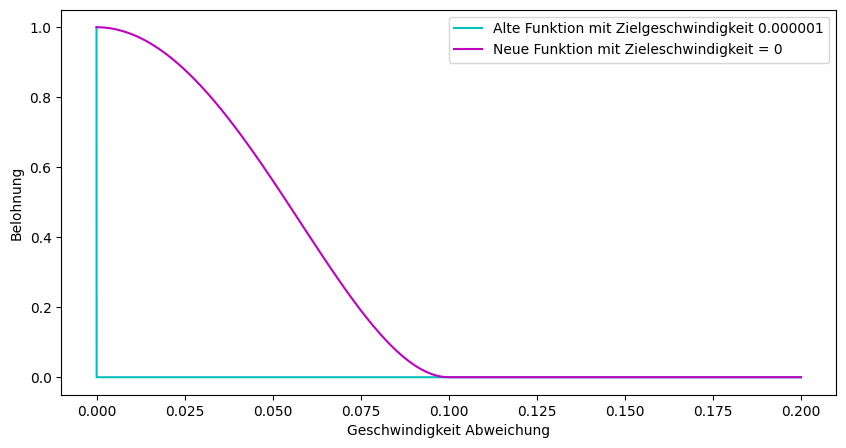
\includegraphics[scale=0.5]{img/match_velocity_vergleich_clip.png}
  \caption{Vergleich Demo gegen Belohnungsfunktion mit 0.1 Limit}
  \label{fig:match_velocity_vergleich_clip}
\end{figure}
$V_\delta=Clip(|\vec{Geschwindigkeit} - \vec{Zielgeschwindigkeit}|, 0, |\vec{Zielgeschwindigkeit}|)$ \\
$V_\delta=Clip(|\vec{Geschwindigkeit} - \vec{Zielgeschwindigkeit}|, 0, max(0.1, |\vec{Zielgeschwindigkeit}|))$ \\

Das auf einer Stelle stehen hat der Läufer damit in einem separaten Training auch erlernt. Abbildung \ref{fig:versuch5_training} zeigt das der Läufer die maximale Episoden Länge von 1000 erreicht hat ohne zu fallen. Die bewegte Distanz hat sich auch 0 angenähert.

\begin{figure}[H]
  \centering  
  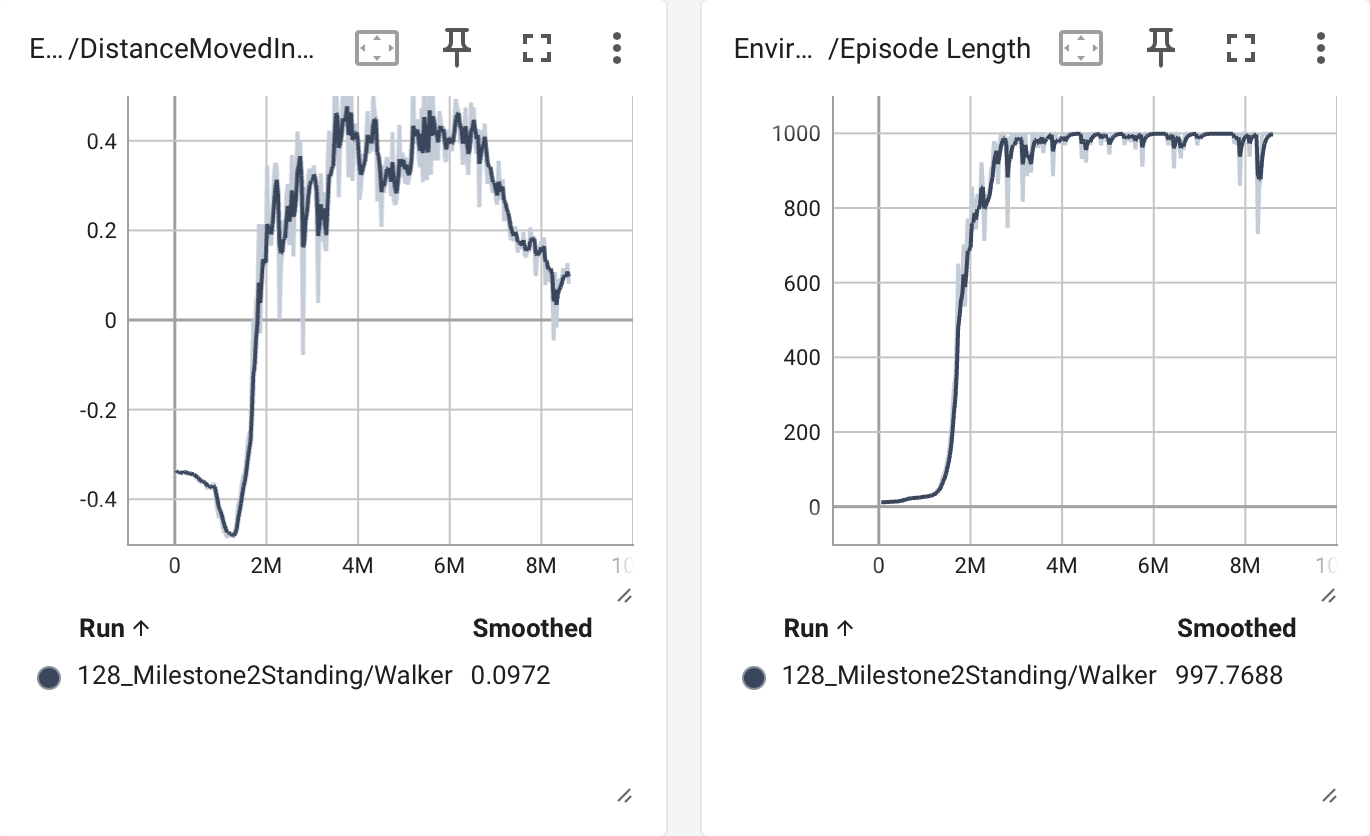
\includegraphics[scale=0.5]{img/versuch5_training.png}
  \caption{Versuch 5 Traininggraphen}
  \label{fig:versuch5_training}
\end{figure}

Die Belohnungen wurden auch weitestgehend optimiert siehe Abbildung \ref{fig:versuch5_training_belohnung}.

\begin{figure}[H]
  \centering  
  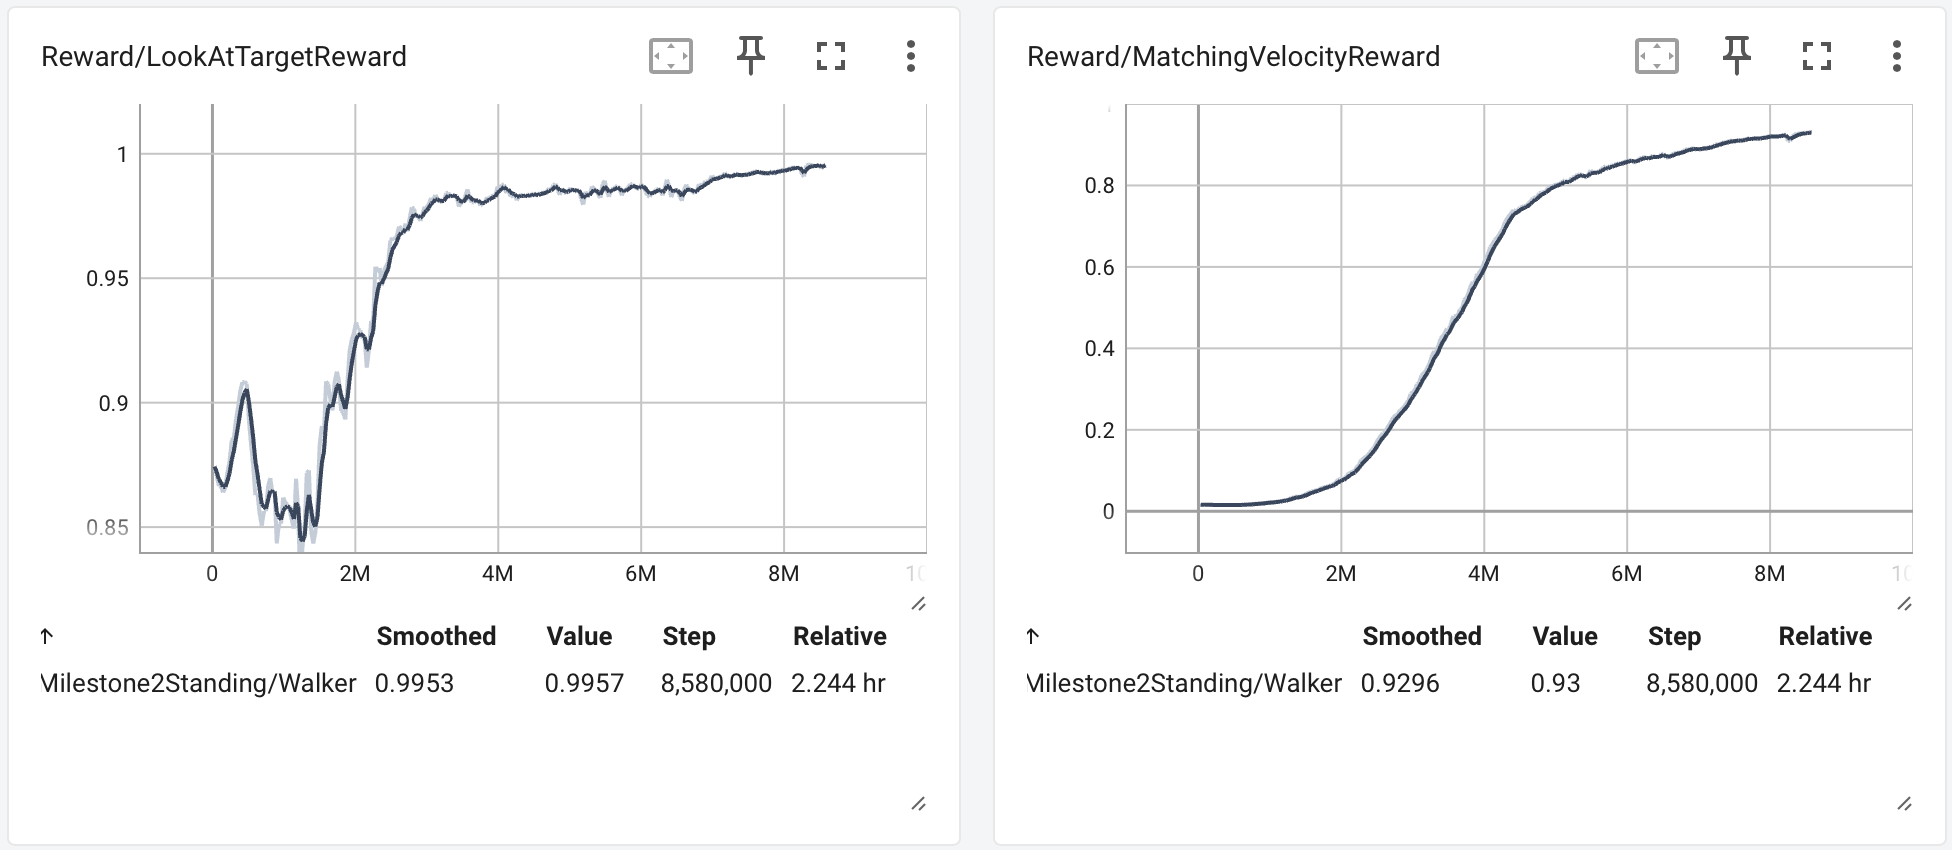
\includegraphics[scale=0.5]{img/versuch5_training_belohnung.png}
  \caption{Versuch 5 Training Belohnungsgraphen}
  \label{fig:versuch5_training_belohnung}
\end{figure}

\subsection{Versuch 6}
Der folgende Versuch untersucht das Laufen in unterschiedliche Richtungen relativ zur Blickrichtung. Um das zu realisieren wurde dem Agent ein enum mit der Laufrichtung hinzugefügt. Die Blickrichtung Belohnungsfunktion wird relativ zur Zielrichtung berechnet. Bei Vorwärtsbewegung ist die Blickrichtung gerade aus. Bei Seitlicher Bewegung ist die Blickrichtung gespiegelt zur Laufrichtung. Läuft der Läufer seitlich rechts ist die Blickrichtung links zum ziel und anders herum. Beim rückwärts gehen ist die Blickrichtung entgegen der Zielrichtung. Die Implementierung ist in \ref{lst:laufrichtung} zu sehen.

\begin{lstlisting}[caption={Laufrichtung Enum, Beobachtung und Belohnung},captionpos=b,label={lst:laufrichtung}]
public enum Direction
{
    Forward,
    Right,
    Left,
    Backward,
}
    
public override void FixedUpdate()
{
    ...
    var headForward = head.forward;
    headForward.y = 0;
    Vector3 lookDirection = cubeForward;
    switch (direction)
    {
        case Direction.Right:
            lookDirection = -walkOrientationCube.transform.right;
            break;
        case Direction.Left:
            lookDirection = walkOrientationCube.transform.right;
            break;
        case Direction.Backward:
            lookDirection = -walkOrientationCube.transform.forward;
            break;
    }
    ...
}
\end{lstlisting}

Das gehen in Zielrichtung wurde durch die Änderungen nicht beeinflusst. Separate Trainings zu den drei anderen Laufrichtungen waren erfolgreich.

\begin{figure}[H]
  \centering  
  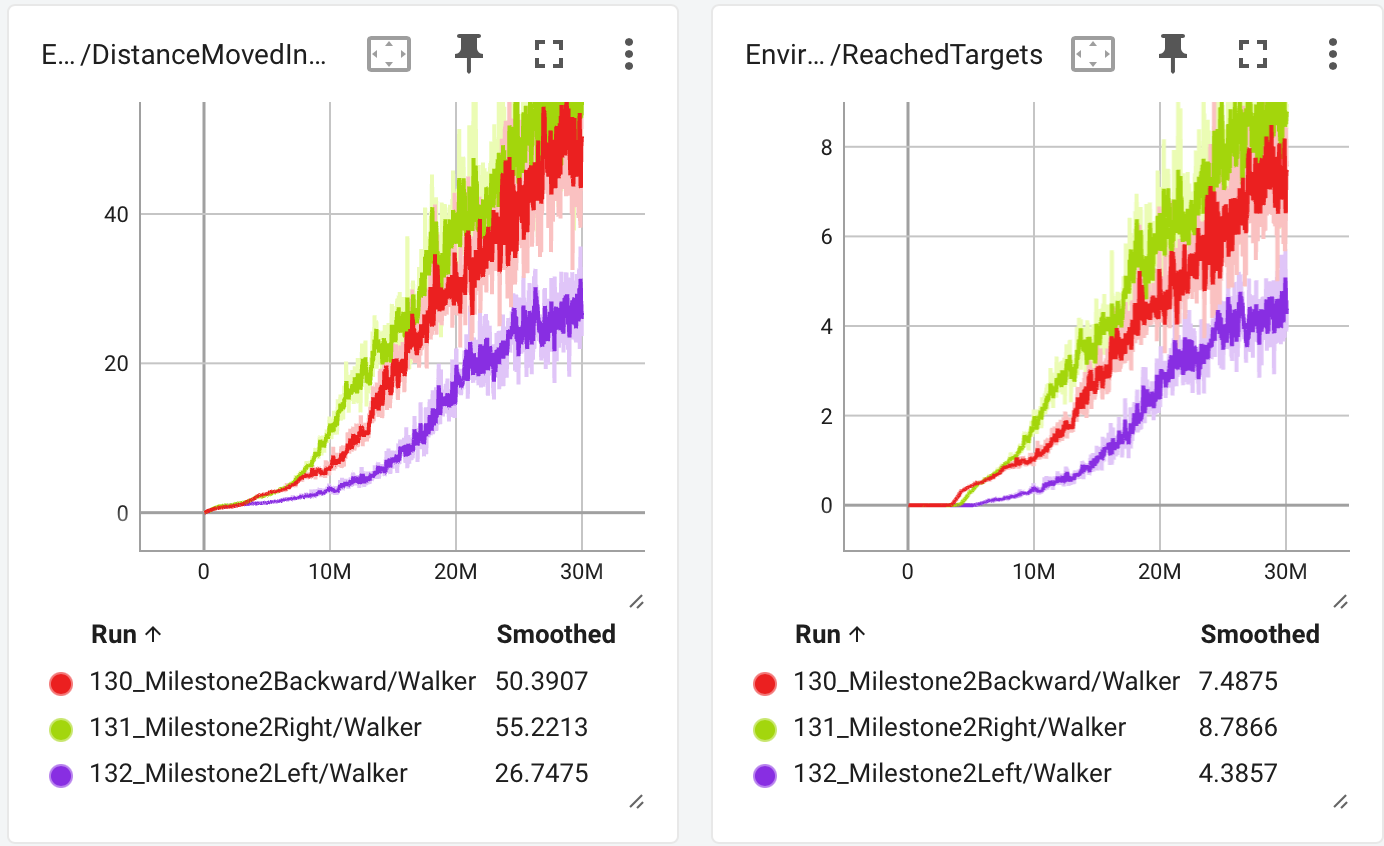
\includegraphics[scale=0.5]{img/versuch6_training.png}
  \caption{Versuch 6 Traininggraphen}
  \label{fig:versuch6_training}
\end{figure}

Abbildung \ref{fig:versuch6_training} zeigt die zurückgelegte Distanz und die Anzahl an erreichten Zielen in einer Trainingsepisode. Die Ergebnisse der 3 Laufrichtungen (rot = Rückwärts, gelb = rechts, blau = links) sind alle vergleichbar mit den Ergebnissen der Demo. Die Abweichung der Laufrichtung Links ist vermutlich der zufällligen Natur des Trainings anzurechnen.

\subsection{Versuch 7}